Finalment, amb tots els problemes degudament identificats i solucionats amb els dos primers prototips, es van dissenyar i construir dos prototips, anomenats TRITIUM-Aveiro i TRITIUM-IFIC-2, amb un disseny funcional i optimitzat per a la detecció del triti. 

Aquests dos presenten un disseny similar que consisteix en un atuell de PTFE a l'interior del qual se situen les fibres centellejadores. Per permetre la utilització d'un gran nombre de fibres (cents) aquestes es van situar lliurement dins atuell, prescindint de la matriu de PTFE. Aquesta llibertat permet el flux de l'aigua a través de les fibres. A més, es van realitzar coincidències temporals entre dos PMTs acoblats amb greix òptic a cada extrem de les fibres, necessari per reduir el fons radioactiu tant com sigui possible. Per poder realitzar de forma segura aquesta coincidència temporal va ser necessari introduir al atuell dues finestres de polimetilmetacrilat (PMMA) que permetessin als fotons generats a les fibres (dins del atuell) arribar fins als PMTs (fora del atuell). Els PMTs utilitzats en cada prototip són el model R$2154-02$ de Hamamtsu \cite{DataSheetPMTsAveiro} per a TRITIUM-Aveiro (el qual conté 360 fibres) i el model R$8520-06SEL$ de Hamamatsu \cite{DataSheetPMTs} per a TRITIUM-IFIC-2 (el qual conté 800 fibres).

Aquests dos prototips presenten diferències subtils en els dissenys. Entre les més importants es troben:

\begin{enumerate}

\item{} El diàmetre de les fibres utilitzades en cada prototip, $2~\mm$ per a les utilitzades en TRITIUM-Aveiro i $1~\mm$ per a les utilitzades en TRITIUM-IFIC-2. Un diàmetre més gran li confereix una major rigidesa al prototip i millora el flux de l'aigua a través de les fibres. No obstant això, també implica una relació senyal-fons menor, donant lloc a una eficiència més baixa i, per tant, a una MDA per al triti més alta.

\item{} A més, el protocol de tractament de la superfície de les fibres centellejadores, comentat a la secció \ref{subsec:Fibres}, no va ser aplicat a les fibres utilitzades en el prototip TRITIUM-Aveiro ja que aquest encara no estava desenvolupat. Com s'ha provat amb tests experimentals, aquest tractament millora la intensitat del senyal en més d'un factor dos, que a causa dels xicotets senyals electrònics generats pels esdeveniments del triti implica una millora substancial en l'eficiència de detecció.


\item{} L'ús de fotosensors diferents. El prototip TRITIUM-Aveiro utilitza dos PMT en coincidència temperal mentre que la proposta per al prototip de TRITIUM-IFIC-2 és utilitzar matrius de SiPMs. Els SiPM tenen una major eficiència de fotodetecció, que dona com a resultat una major eficiència en la detecció del triti. No obstant això, aquests presenten un soroll electrònic més alt, incrementant el fons radioactiu mesurat pel detector. %Cal tenir en compte que aquesta serà una diferència per al futur ja que, fins ara, les mesures han estat preses sols amb PMTs. 

\end{enumerate} 

Totes aquestes opcions seran provades i aquelles amb millors resultats seran implementades al prototip final. El disseny d'aquests prototips es mostren a la figura \ref{fig:PrototipsAveiroIFIC2}.

\begin{figure}
\centering
    \begin{subfigure}[b]{0.5\textwidth}
    \centering
    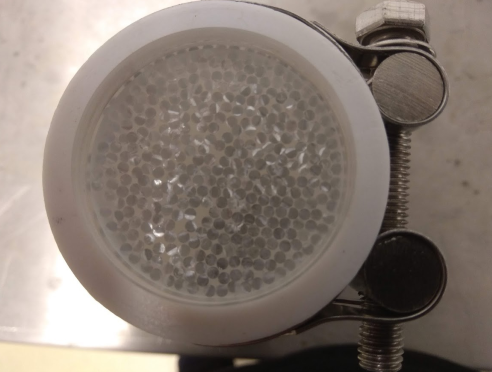
\includegraphics[width=\textwidth]{12Summary/5Prototypes/53FinalPrototypes/531TritiumAveiro/TeflonVessel_Fibers.png}  
        \caption{}\label{subfig:PrototipAveiro}
    \end{subfigure}
    \hfill
    \begin{subfigure}[b]{0.5\textwidth}
    \centering
    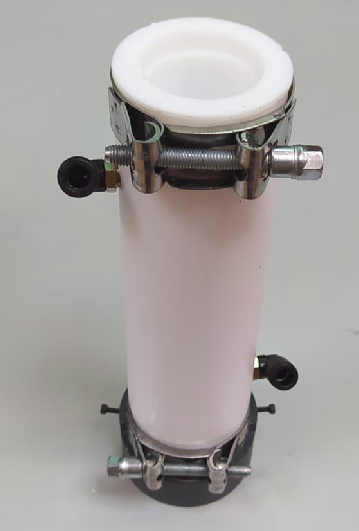
\includegraphics[width=\textwidth]{12Summary/5Prototypes/53FinalPrototypes/532TritiumIFIC2/Tritium_IFIC_2_vessel1.png}  
    \caption{\label{subfig:PrototipIFIC2}}
    \end{subfigure}
\caption{a) Prototip TRITIUM-Aveiro. b) Prototip TRITIUM-IFIC-2. \label{fig:PrototipsAveiroIFIC2}.}
\end{figure}

L'objectiu d'aquests prototips no és trobar problemes en el disseny sinó mesurar l'eficiència en la detecció del triti i la MDA. Per tant, l'activitat de la dissolució d'aigua tritiada utilitzada en aquests va ser inferior, $30$ i $10~\kilo\becquerel/\liter$ per als prototips TRITIUM-Aveiro i TRITIUM-IFIC-2 respectivament.

Els espectres d'energia mesurats amb el prototip TRITIUM-IFIC-2 i les respectives taxes de comptatge mesurades són  mostrats a la Figura \ref{fig:EspectresEnergeticsTRITIUMIFIC2} i a la Taula \ref{tab:ContesPerSegonTRITIUMIFIC2}, respectivament. El prototip TRITIUM-Aveiro utilitza una electrònica diferent que mesura directament la taxa de comptatge sense la necessitat d'obtenir els espectres d'energia. aquests són també mostrats a la Taula \ref{tab:ContesPerSegonTRITIUMIFIC2}.

\begin{figure}
\centering
    \begin{subfigure}[b]{1\textwidth}
    \centering
    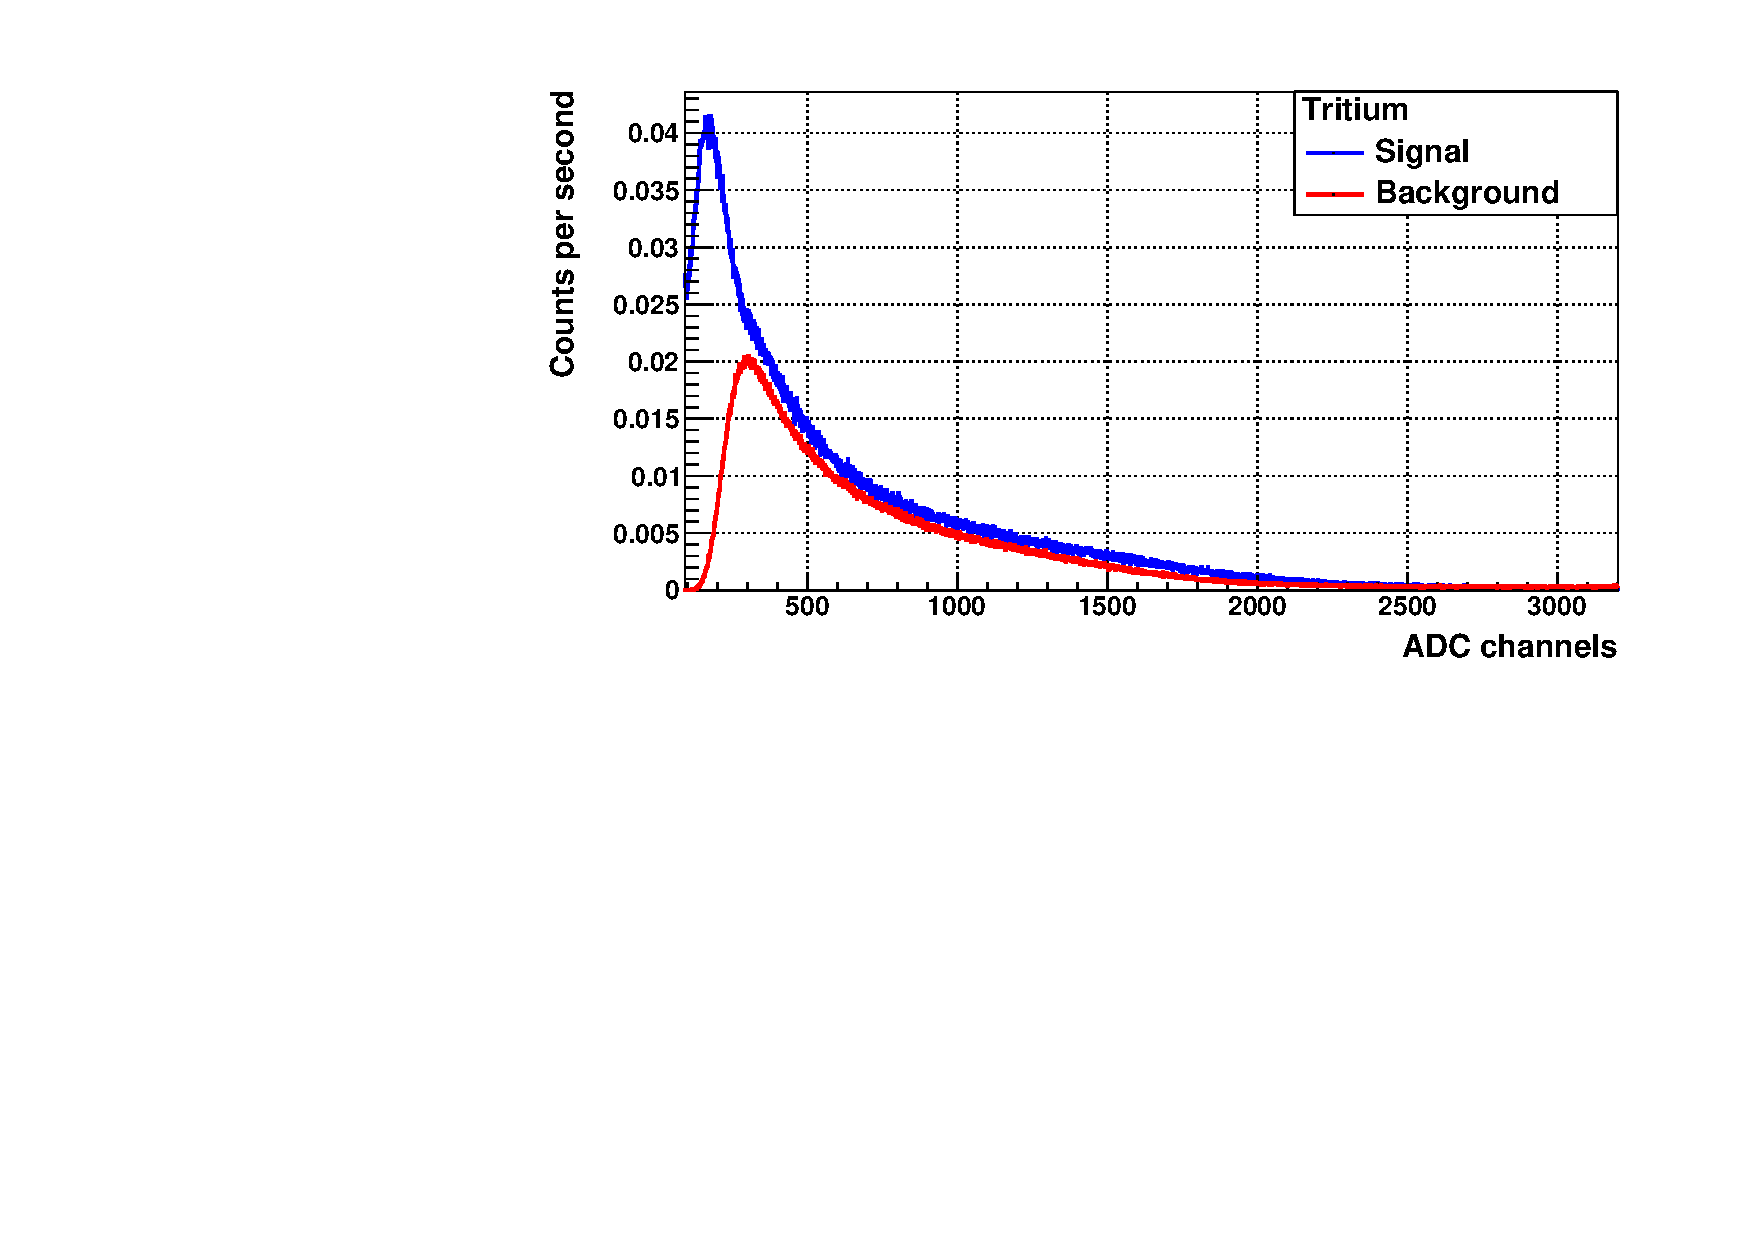
\includegraphics[width=\textwidth]{12Summary/5Prototypes/53FinalPrototypes/532TritiumIFIC2/TritiumIFIC2SignalsHigherZOOM_NP.pdf}  
    \caption{\label{subfig:EspectreEnergeticSenyalFonsTritiumIFIC2}}
    \end{subfigure}
    \hfill
    \begin{subfigure}[b]{1\textwidth}
    \centering
    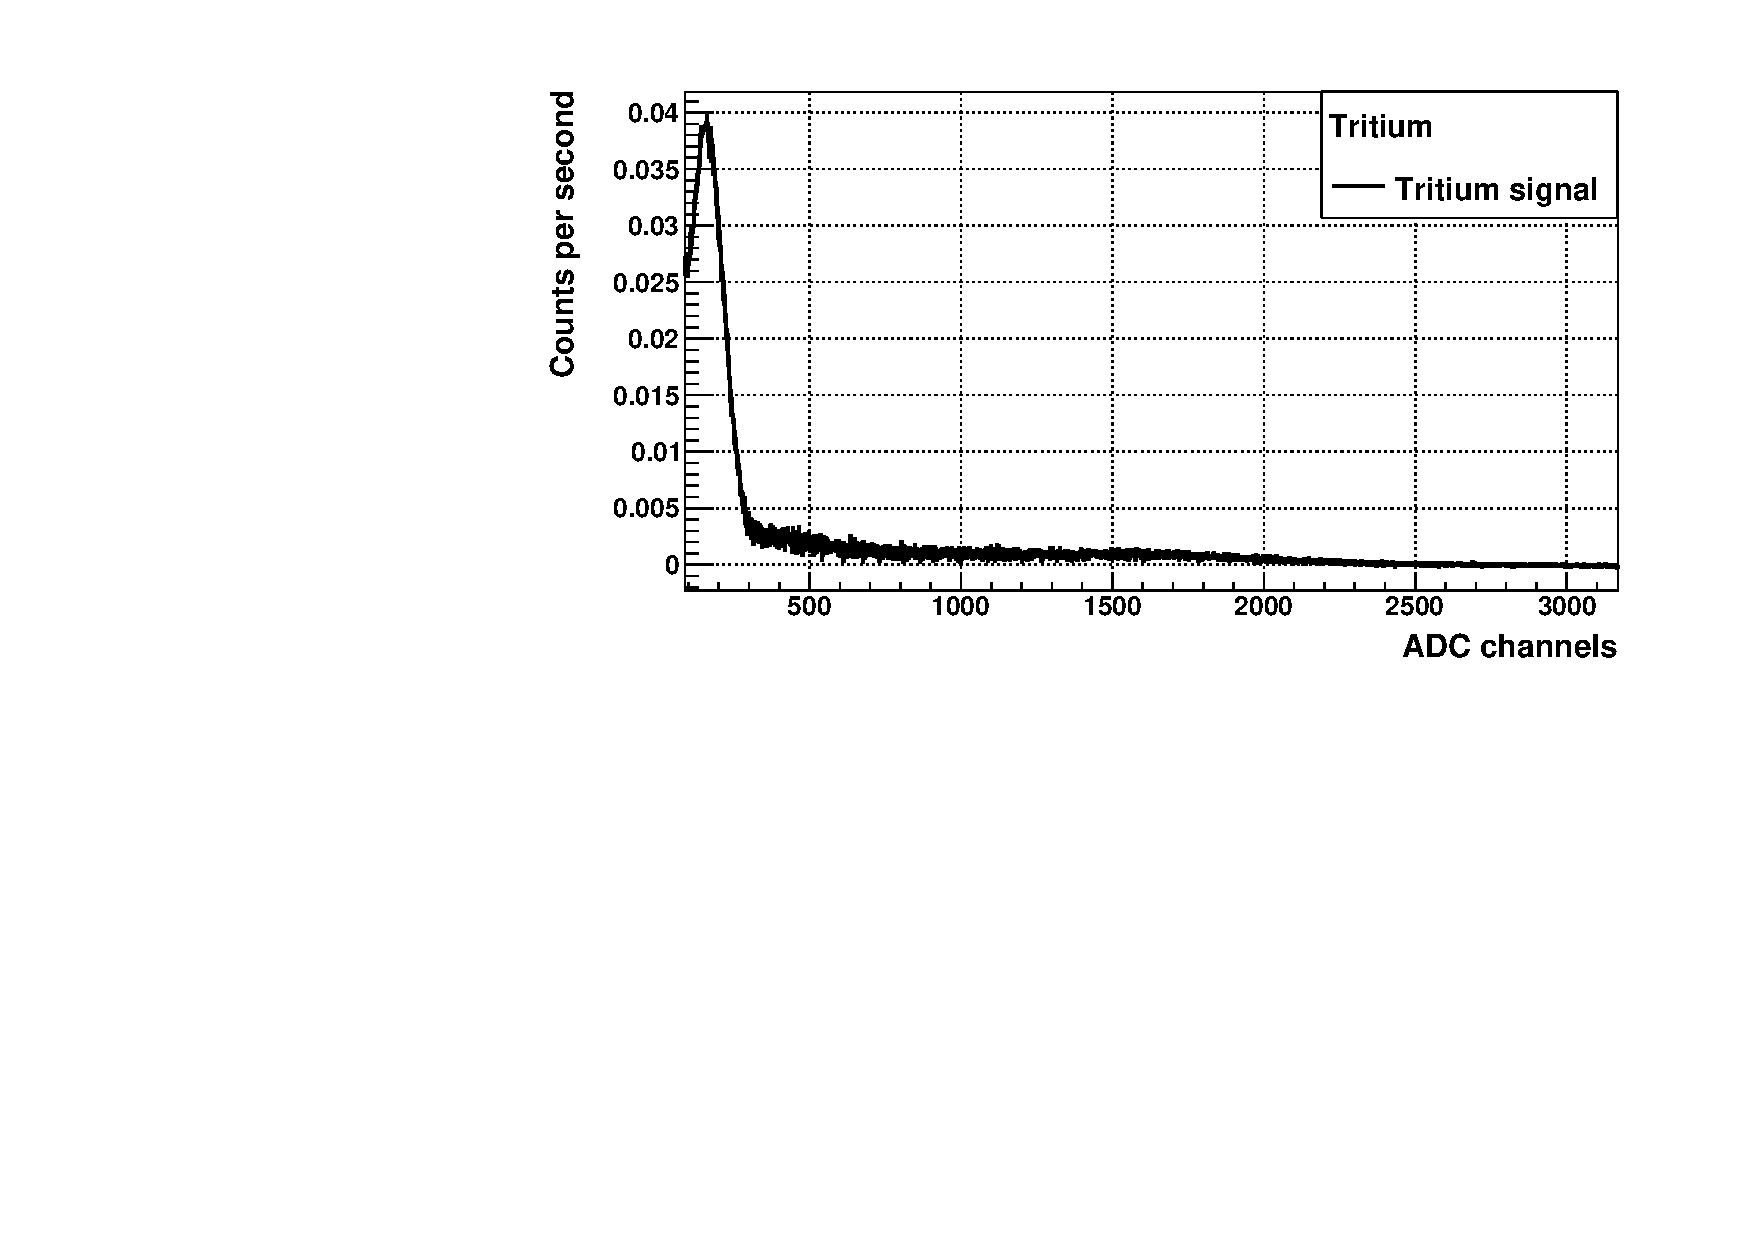
\includegraphics[width=\textwidth]{12Summary/5Prototypes/53FinalPrototypes/532TritiumIFIC2/TritiumIFIC2ClearHigherZOOM_NP.pdf}  
    \caption{\label{subfig:EspectreEnergeticTritiTritiumIFIC2}}
    \end{subfigure}
 \caption{Espectres d'energia mesurats amb el prototip TRITIUM-IFIC-2. a) Espectre d'energia de senyal i fons. b) Espectre d'energia del triti.}
 \label{fig:EspectresEnergeticsTRITIUMIFIC2}
\end{figure}

\begin{table}[htbp]
\centering{}%
\begin{tabular}{ccc}
\toprule 
Espectres & TRITIUM-Aveiro & TRITIUM-IFIC-2  \tabularnewline
\midrule
\midrule 
Prototip del senyal & $10.93 \pm 0.4$ & $19.05 \pm 0.18$ \tabularnewline
Prototip del fons & $9 \pm 0.4$ & $11.54 \pm 0.14$ \tabularnewline  
Espectre de triti & $1.93 \pm 0.58$ & $7.11 \pm 0.23$ \tabularnewline
\bottomrule
\end{tabular}
\caption{Taxes de comptatge mesurades amb el prototip TRITIUM-IFIC-2.}
\label{tab:ContesPerSegonTRITIUMIFIC2}
\end{table}

L'eficiència específica en la detecció del triti obtinguda per a aquests prototips es
$$S = (1.6 \pm 0.5)\cdot{} 10^{-5}~\frac{cps}{\kilo\becquerel/\liter \cdot{} \cm^{2}}$$
$$S = (14.1 \pm 0.6)\cdot{} 10^{-5}~\frac{cps}{\kilo\becquerel/\liter \cdot{} \cm^{2}}$$
per a TRITIUM-Aveiro i TRITIUM-IFIC-2, respectivament. Com es pot observar l'eficiència obtinguda per al prototip TRITIUM-IFIC-2, millora l'obtinguda amb els prototips anteriors i els detectors de triti similars desenvolupats fins ara en altres col·laboracions \cite{Hofstetter1, Hofstetter2}. Veiem per tant que aquest ha superat l'estat actual de l'art de la detecció de triti en l'aigua utilitzant plàstics centellejadors. No obstant això, trobem una eficiència específica inferior a l'esperada per al prototip TRITIUM-Aveiro. Tot indica que aquest resultat és causat principalment pel fet de no aplicar el tractament de la superfície a les fibres centellejadores, algo que deu ser estudiat amb mes deteniment.

Finalment s'aplica el criteri de Currie \cite{Knoll} a tots dos prototips per obtenir la mínima activitat de triti mesurable per cadascun. Els valors obtinguts són $5$ i $0.218~\kilo\becquerel/\liter$ per a mesures d'una hora per al prototip de TRITIUM-Aveiro i TRITIUM-IFIC-2 respectivament. 

L'estabialitat de l'eficiència del prototip TRITIUM-IFIC-2 al llarg del temps es va comprovar fent mesures al llarg de mesos, les quals es mostren a la Figura \ref{fig:MonitoritzacioTRITIUMIFIC2}. Com es pot observar, no s'aprecia cap decaïment durant els sis mesos de mesura, obtenint-se un comportament estable del detector amb una desviació estàndard relativa del $2,5\%$

\begin{figure}[h]
\centering
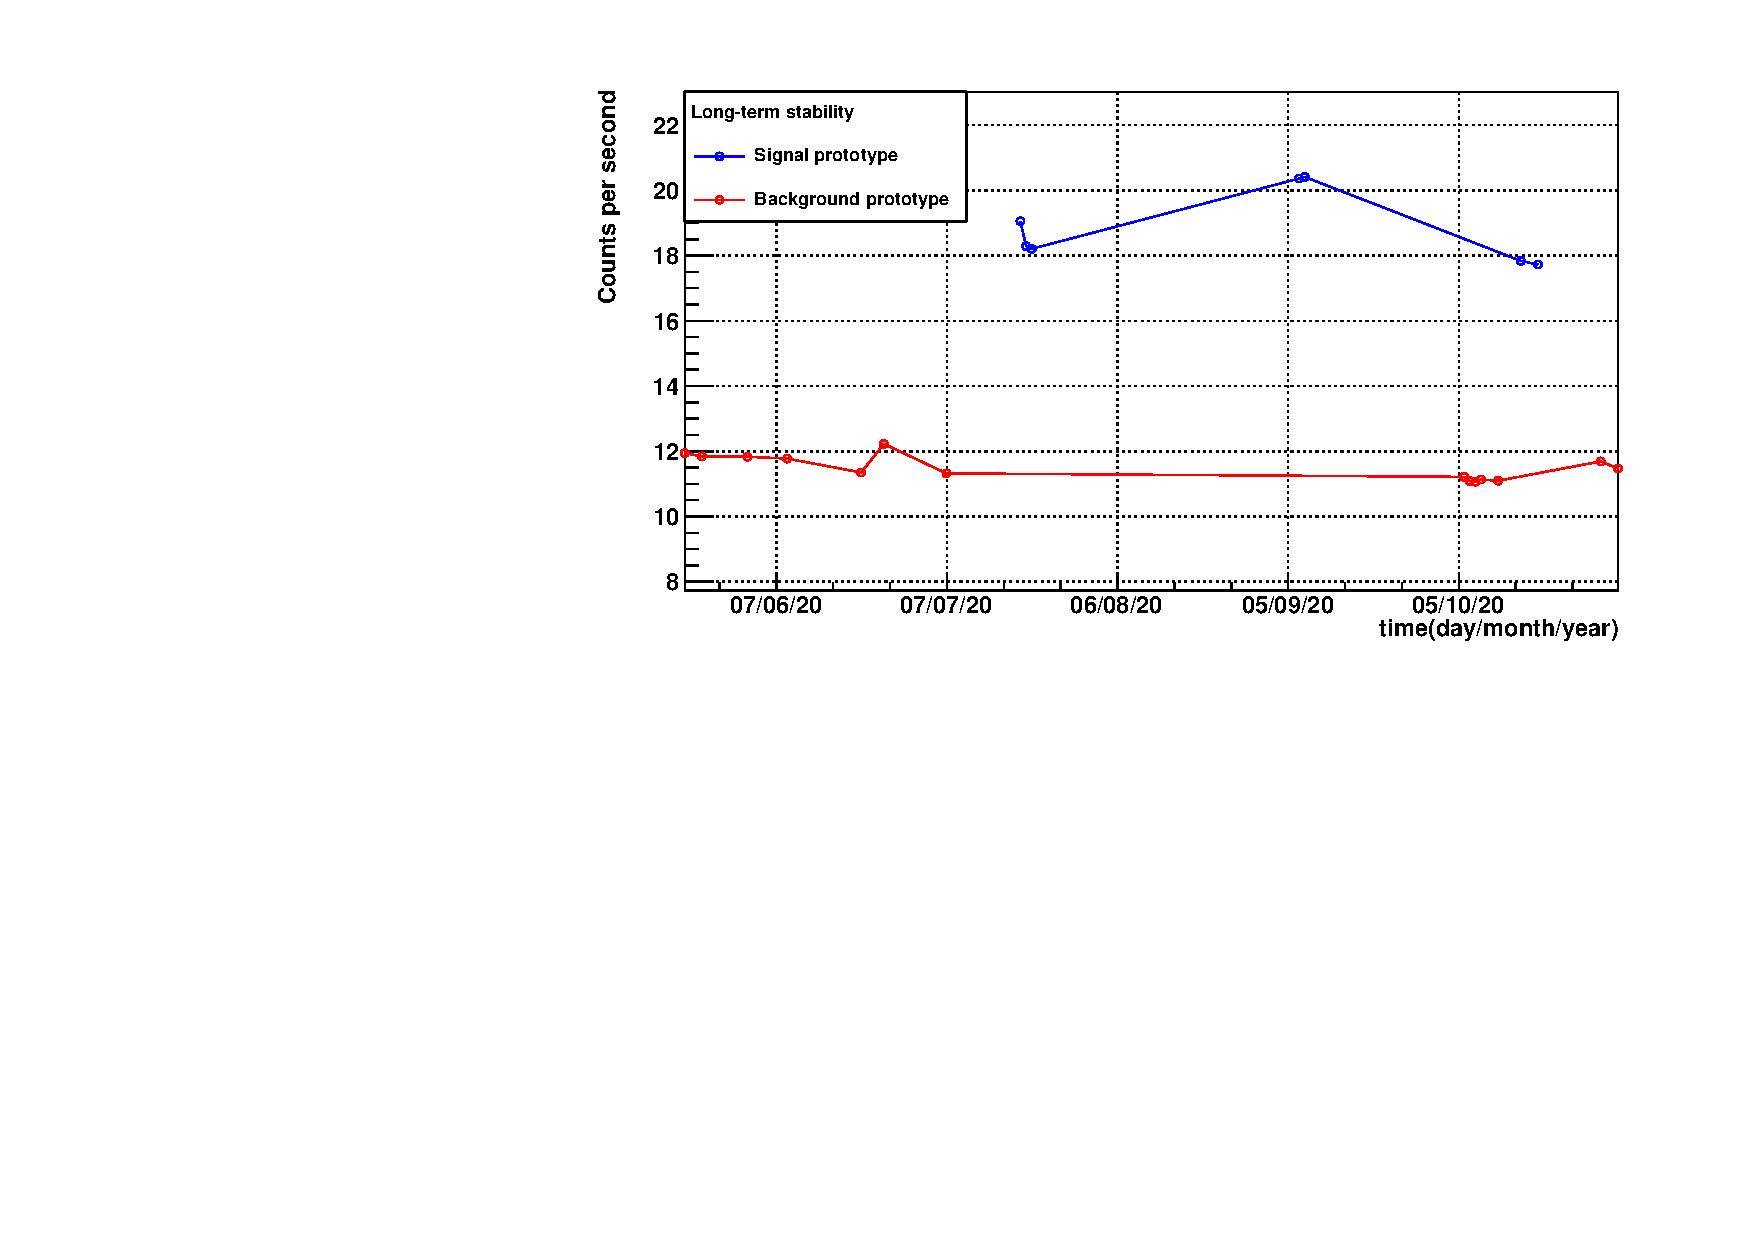
\includegraphics[scale=0.6]{12Summary/5Prototypes/53FinalPrototypes/532TritiumIFIC2/Signal_Background_stability_ZOOM.pdf}
\caption{Taxes de comptatge mesurades amb el prototip TRITIUM-IFIC-2 de fons i senyal al llarg de diversos mesos.\label{fig:MonitoritzacioTRITIUMIFIC2}}
\end{figure}

El prototip TRITIUM-Aveiro es va instalar en Arrocampo el 27 de Març de 2019 i ha estat prenent mesures del fons radioactiu durant mes de cuatre mesos, fins el 18 de Agost de 2019. En aquestes mesures, mostrades a la Figura \ref{fig:FonsArrocampoAveiro}, es pot observar una gran estabilitat al voltant de $9.31$ contes per segón. També s'observa un pic el día 2 de Maig degut a una opertura del castell de plom.

\begin{figure}[h]
\centering
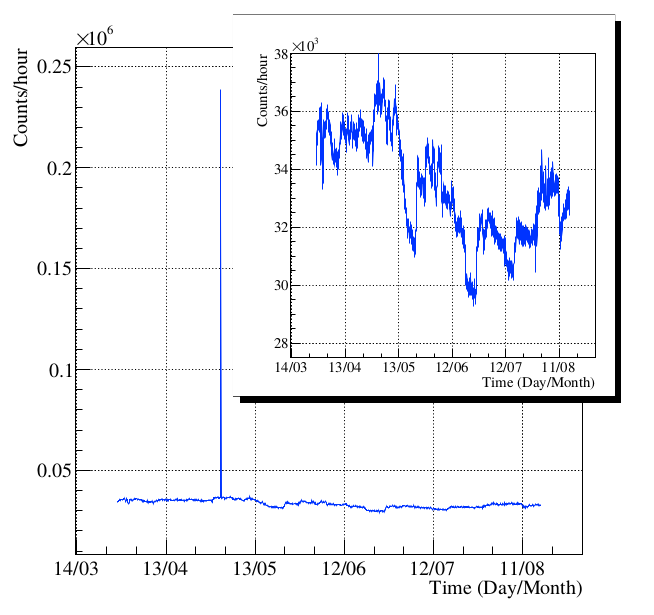
\includegraphics[scale=0.45]{12Summary/5Prototypes/54ArrocampoMeasurements/721TRITIUMAVEIRO0/BackgroundMeasurements.png}
\caption{Mesures del fons radioactiu d'Arrocampo obtingudes amb el prototip TRITIUM-Aveiro.\cite{ExperimentalPaperCarlos}.\label{fig:FonsArrocampoAveiro}}
\end{figure}